\section{Dettagli implementativi}\label{sec:implementazione}
In questo paragrafo verranno descritti in modo specifico i dettagli implementativi di ogni modello e di ogni sua versione, oltre ai vari passaggi di pre-processing e il metodo di valutazione.

\subsection{Pre-processing}
Per le versioni 1 dei modelli i dati non vengono pre-processati, infatti i dati non vengono pre-processati come descritto nella sezione \ref{sec:analisi}, ma vengono solamente fatte le modifiche in fase di EDA, modificando quindi i tipi dei dati ed eliminando i valori NaN. Lo splitting in questo caso è fatto quindi sui dati originali, togliendo dalle features lo \textit{user}, che è il nome del soggetto e non influisce sull'apprendimento, ed è stato tolta anche la feature \textit{gender}, in quanto non ancora trasformata con l'encoder. Inoltre la variabile target \textit{class} in questo caso rimane sottoforma di stringa.

Per le versioni 2 invece vengono effettuati gli step di pre-processing descritti brevemente nella sezione \ref{sec:analisi}, in particolare dopo aver fatto l'encoding della feature \textit{gender} e del target \textit{class}, è stata studiata la matrice di correlazione, mostrata in figura \ref{fig:corr}, per valutare la collinearità tra features tra di loro, e con la variabile target. Ne risulta che le variabili \textit{y1} e \textit{y4} sono particolarmente correlate con la variabile target, quindi saranno importanti ai fini della classificazione. In secondo luogo è possibile notare che le features \textit{how\_tall\_in\_meters}, \textit{weight} e \textit{body\_mass\_index} sono particolarmente correlate tra di loro e di conseguenza è conveniente eliminarne due mantenerne una sola. Infine le tre variabili che rappresentano le coordinate dell'accelerometro 2, quello sulla coscia sinistra, sono molto correlate tra loro, quindi anche in questo caso conviene mantenerne una sola.

\begin{figure}[ht]
    \centering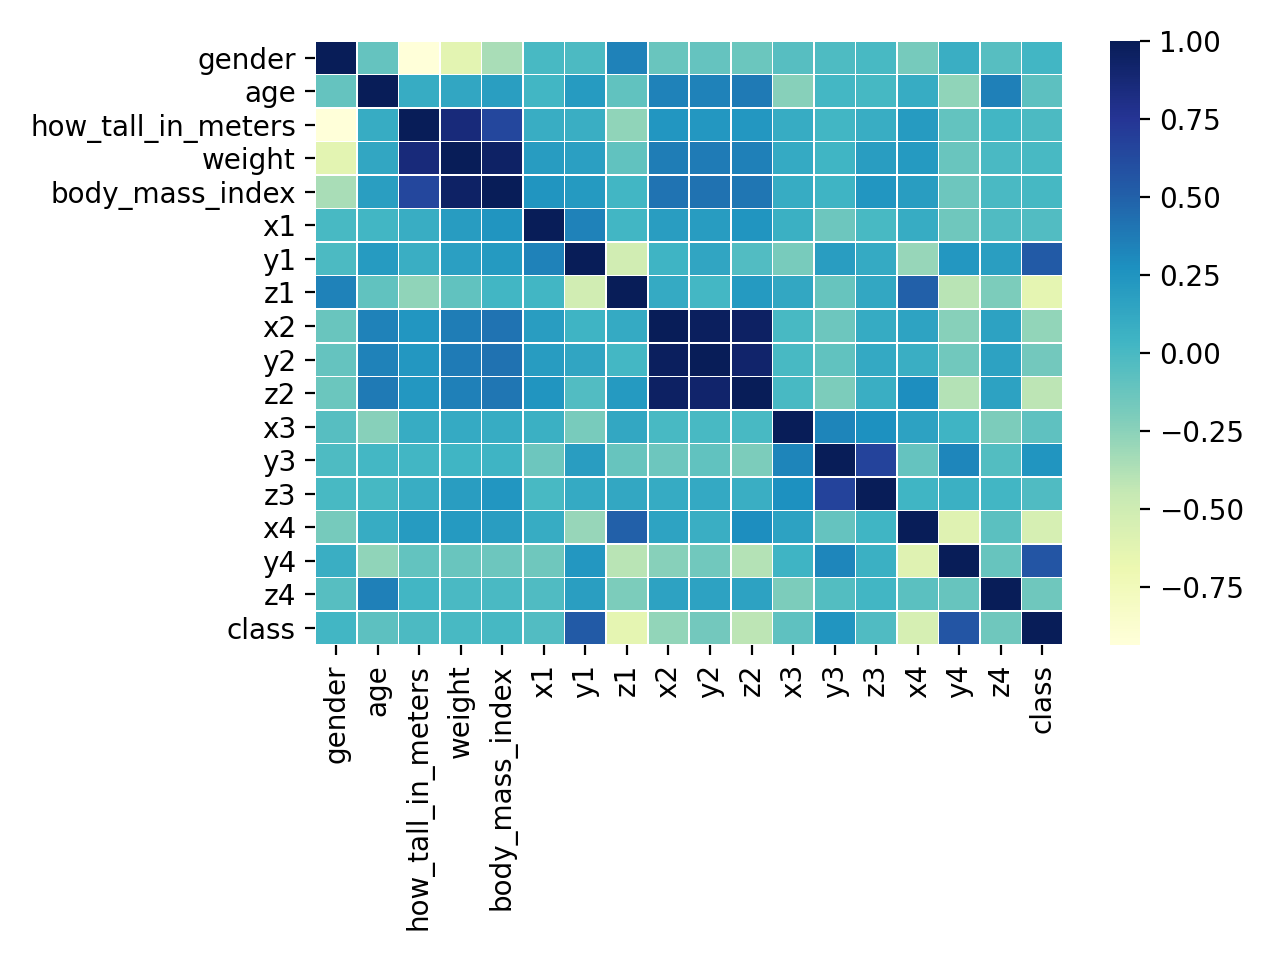
\includegraphics[width=1.0\linewidth]{corr}
    \caption{Matrice di correlazione.}
    \label{fig:corr}
\end{figure}

Dalle informazioni raccolte dalla matrice di correlazione, in figura \ref{fig:corr}, effettuiamo la features selection eliminando le variabili \textit{weight} e \textit{body\_mass\_index} perchè altamente correlate con \textit{how\_tall\_in\_meters} e viene mantenuta quest'ultima; vengono anche eliminate le coordinate x e z del secondo accelerometro, mantenendo solo la coordinata y. Infine vengono eliminate le variabili \textit{user} e \textit{age} in quanto non influenti sul riconoscimento della postura.

Le features selezionate vengono poi sottoposte a uno scaling, in particolare di applica il metodo del \textbf{min-max-scaling}: trasforma il valore di ogni features portandolo a un valore compreso tra 0 e 1, per farlo applica a ogni variabile la seguente formula:

\begin{equation}
x' = \frac{x-min(x)}{max(x)-min(x)}
\end{equation}

È importante sottolineare che i parametri $min(x)$ e $max(x)$ vanno calcolati sulla base del solo training set, dopodiché si applica la trasformazione al training set e al test set.

\begin{figure}[ht]
    \centering
    \begin{subfigure}[t]{0.4\textwidth}
        \centering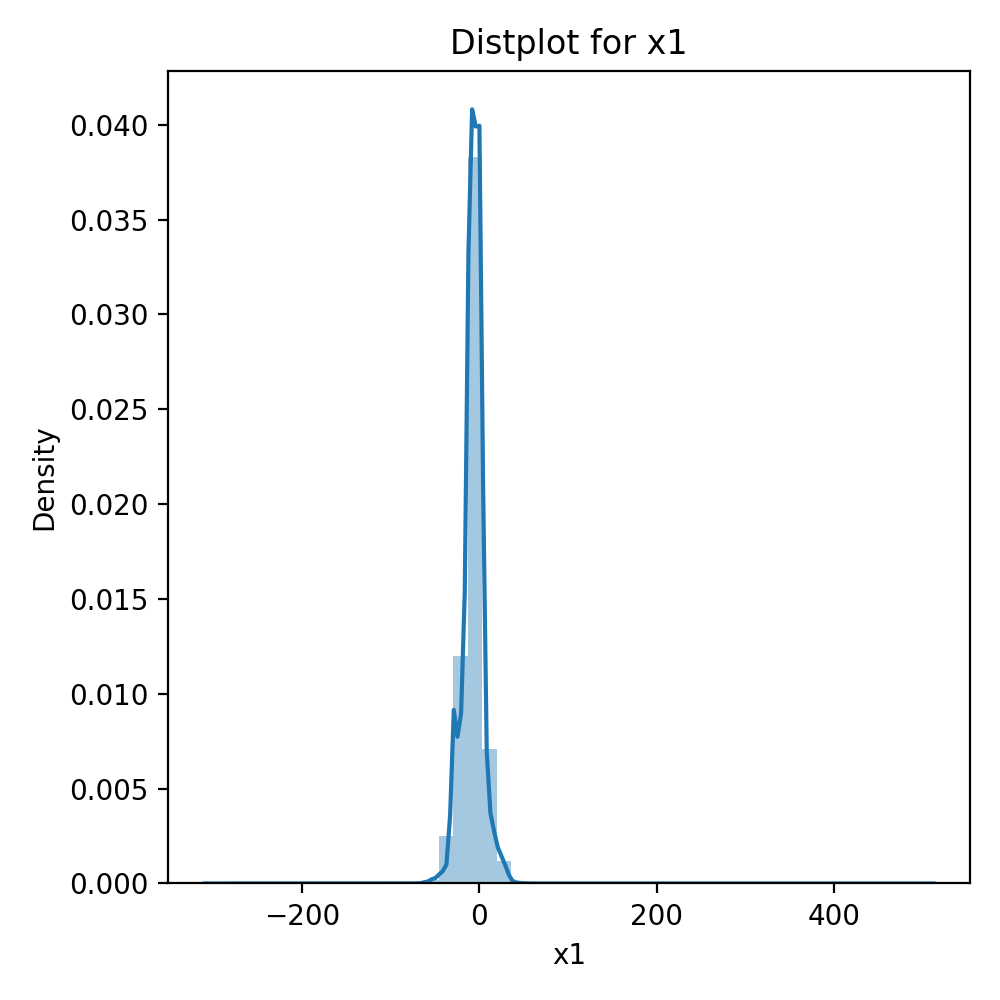
\includegraphics[width=1\linewidth]{x1prescaling}
        \caption{Distribuzione di x1 prima del min-max-scaling.}
        \label{fig:distprescaling:x1}
    \end{subfigure}
    %
    \begin{subfigure}[t]{0.4\textwidth}
        \centering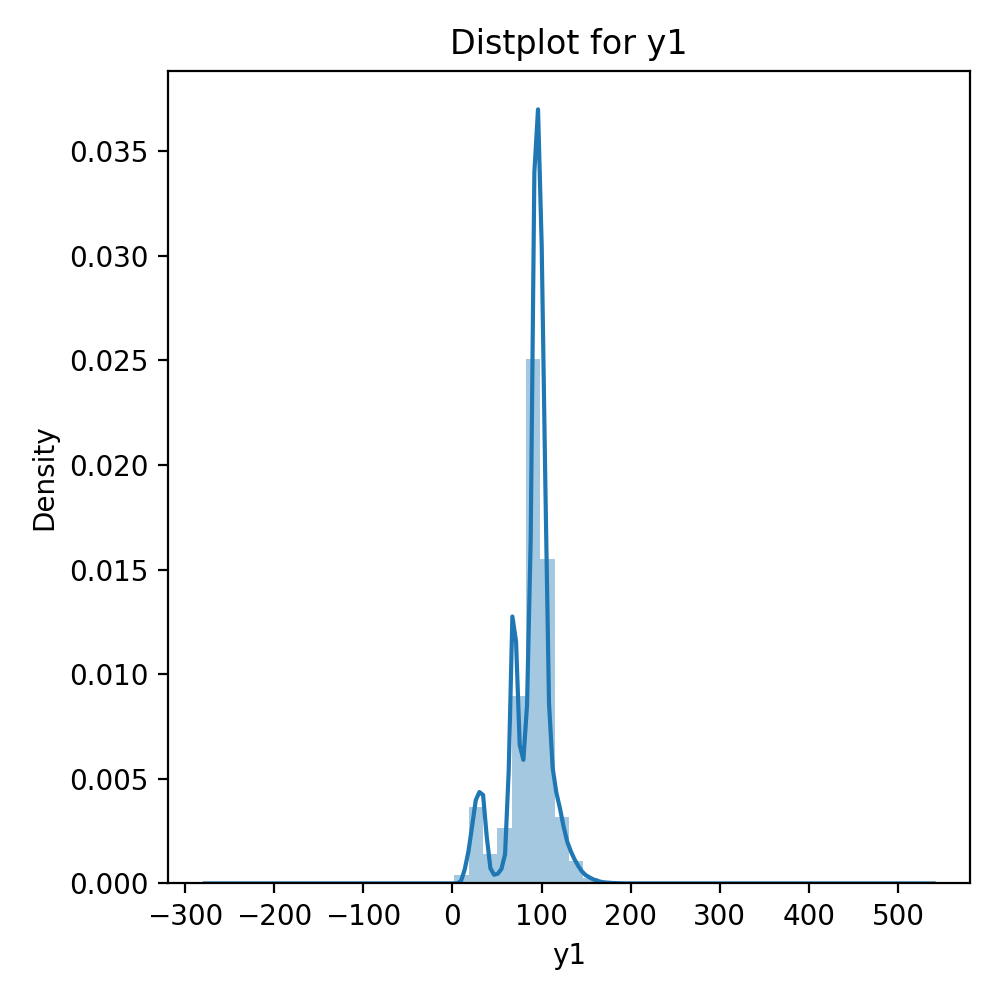
\includegraphics[width=1\linewidth]{y1prescaling}
        \caption{Distribuzione di y1 prima del min-max-scaling.}
        \label{fig:distprescaling:y1}
    \end{subfigure}
    %
    \\
    \begin{subfigure}[t]{0.4\textwidth}
        \centering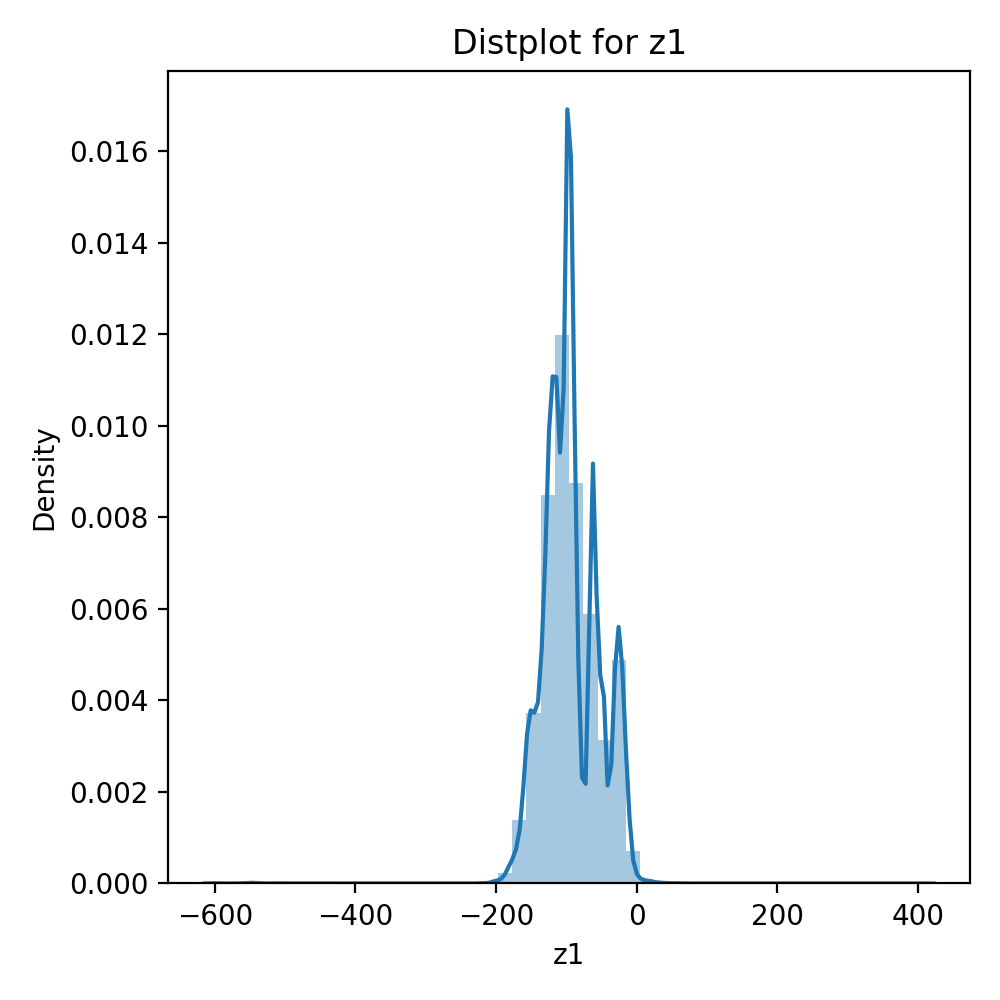
\includegraphics[width=1\linewidth]{z1prescaling}
        \caption{Distribuzione di z1 prima del min-max-scaling.}
        \label{fig:distprescaling:z1}
    \end{subfigure}
    %
    \begin{subfigure}[t]{0.4\textwidth}
        \centering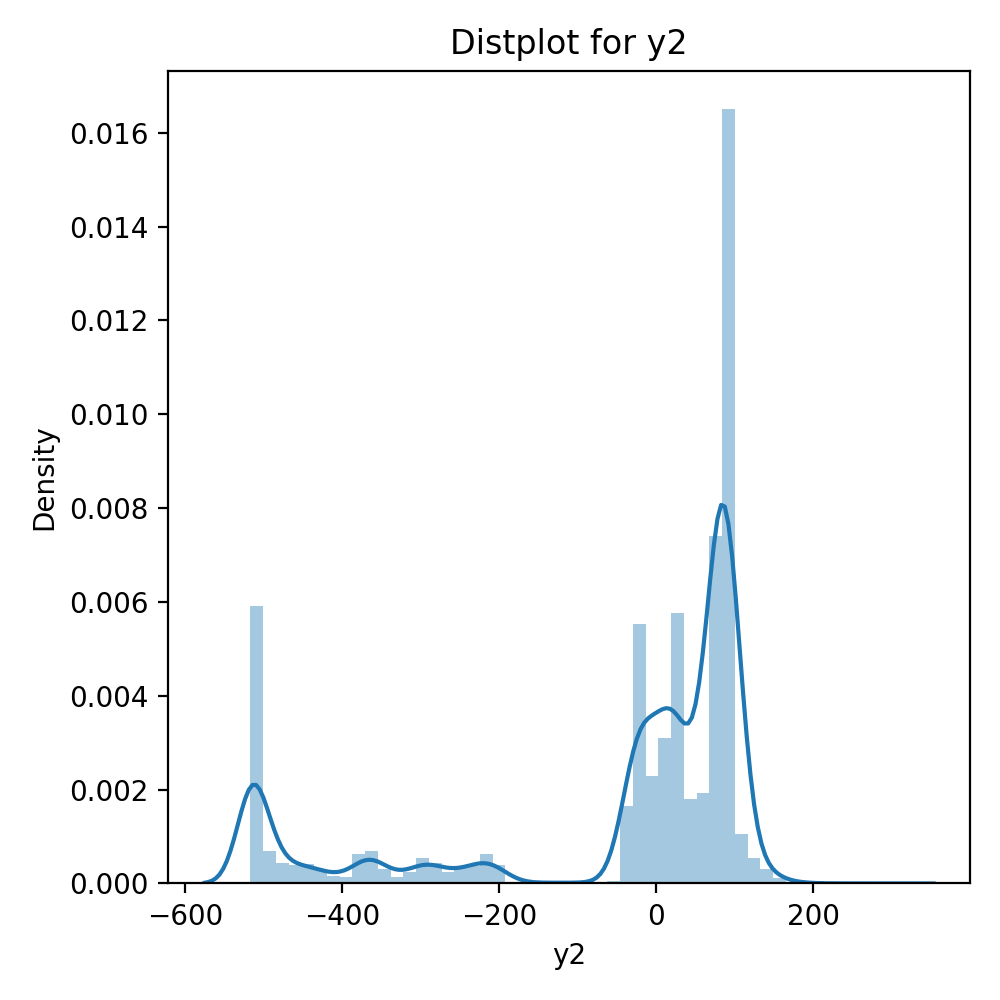
\includegraphics[width=1\linewidth]{y2prescaling}
        \caption{Distribuzione di y2 prima del min-max-scaling.}
        \label{fig:distprescaling:y2}
    \end{subfigure}
    \caption{Distribuzione di variabili prima del min-max-scaling.}
    \label{fig:distprescaling}
\end{figure}

In figura \ref{fig:distprescaling} sono mostrati i grafici di distribuzione di alcune variabili prima di aver subito il min-max-scaling, come si vede i valori variano nell'ordine delle centinaia intorno allo zero.

\begin{figure}[ht]
    \centering
    \begin{subfigure}[t]{0.4\textwidth}
        \centering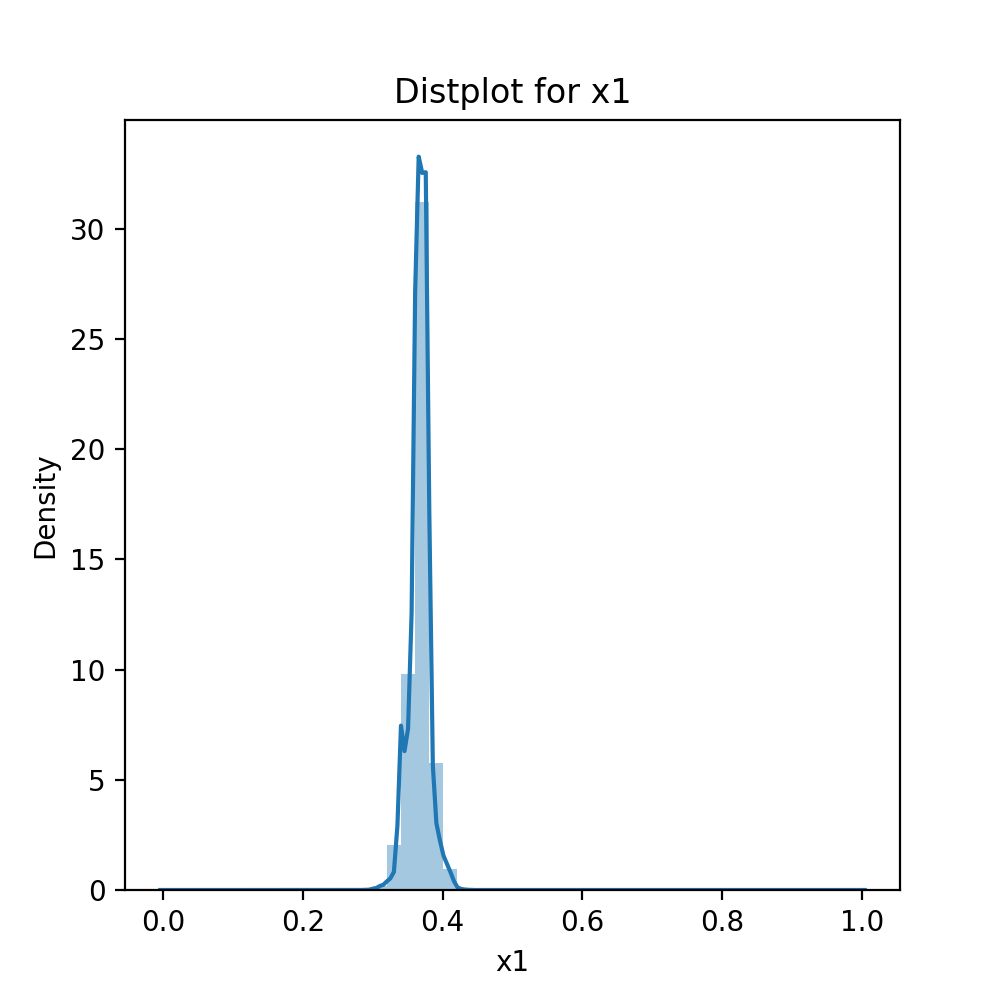
\includegraphics[width=1\linewidth]{x1postscaling}
        \caption{Distribuzione di x1 dopo il min-max-scaling.}
        \label{fig:distpostscaling:x1}
    \end{subfigure}
    %
    \begin{subfigure}[t]{0.4\textwidth}
        \centering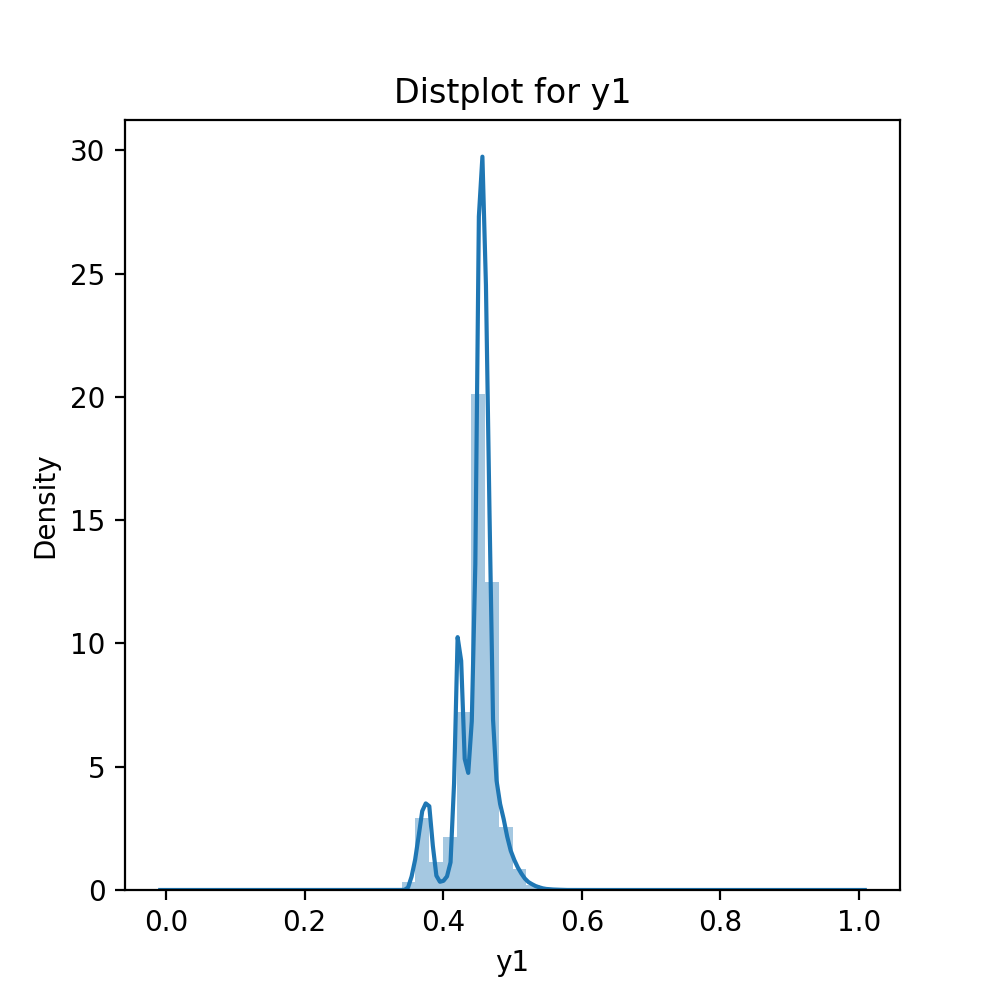
\includegraphics[width=1\linewidth]{y1postscaling}
        \caption{Distribuzione di y1 dopo il min-max-scaling.}
        \label{fig:distpostscaling:y1}
    \end{subfigure}
    %
    \\
    \begin{subfigure}[t]{0.4\textwidth}
        \centering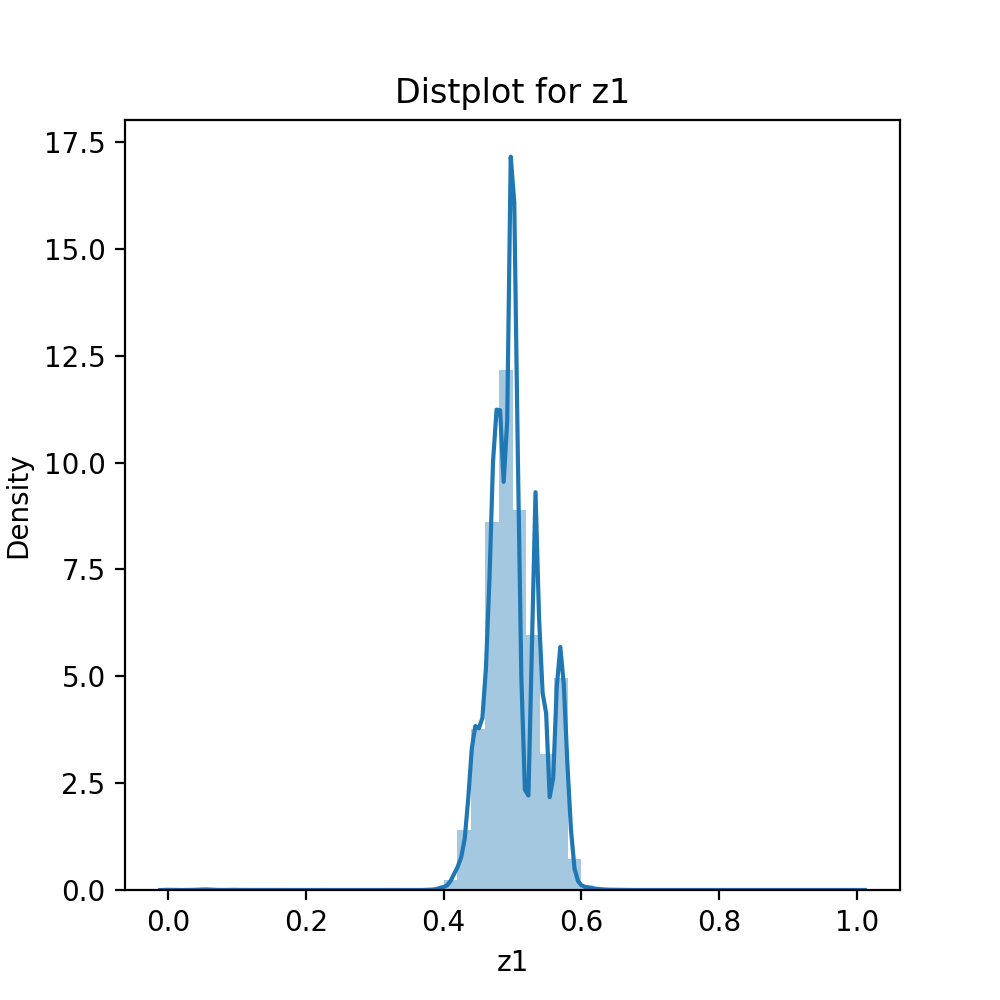
\includegraphics[width=1\linewidth]{z1postscaling}
        \caption{Distribuzione di z1 dopo il min-max-scaling.}
        \label{fig:distpostscaling:z1}
    \end{subfigure}
    %
    \begin{subfigure}[t]{0.4\textwidth}
        \centering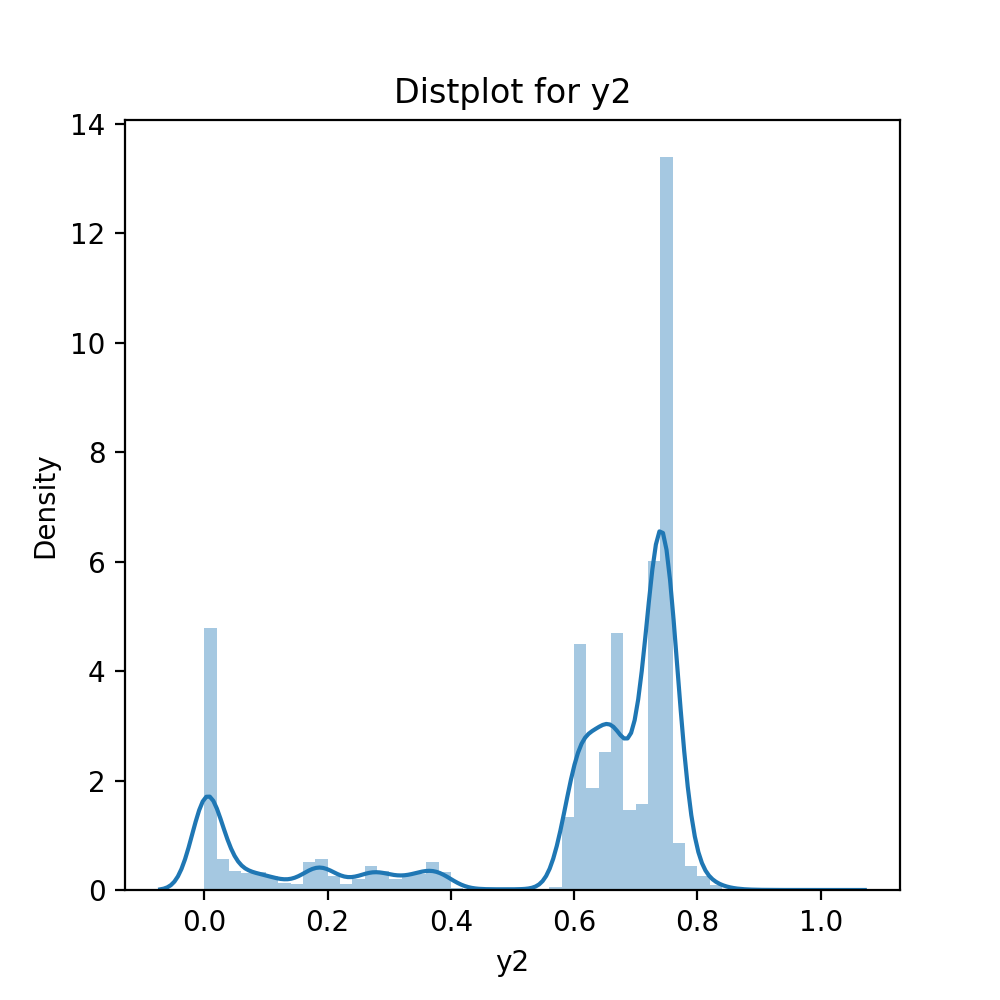
\includegraphics[width=1\linewidth]{y2postscaling}
        \caption{Distribuzione di y2 dopo il min-max-scaling.}
        \label{fig:distpostscaling:y2}
    \end{subfigure}
    \caption{Distribuzione di variabili dopo il min-max-scaling.}
    \label{fig:distpostscaling}
\end{figure}

In figura \ref{fig:distpostscaling} invece sono mostrati i grafici delle distribuzioni delle stesse variabili dopo aver subito la trasformazione del min-max-scaling, come si vede il valore è compreso tra 0 e 1 ma l'andamento è lo stesso e la distribuzione mantiene la stessa forma, a prova del fatto che i dati mantengono le stesse informazioni rappresentative. Grazie a quest'operazione di trasformazione delle features i modelli saranno più efficienti in fase di training e veloci.

\subsection{Decision Tree}

\subsection{Support Vector Machine}

\subsection{Reti neurali}

\subsection{Metriche di valutazione}